\subsection{Calibration}
\label{ref:calibration}

It is unfortunate but neccessary that for this method of vehicle classification that for each different location and camera angle an element of calibration is required to obtain best results. This is a function of the size of vehicles in the camera frame and the lighting conditions at the location. Presently these factors are compensated for by manually calibrating parameters of each subprocess.

\subsubsection{Background Subtractor}

The OpenCV class \emph{BackgroundSubtractorMOG2} has a number of parameters that change the behaviour of a GMM instance. Pertinent to this particular application of the model, vehicle segmentation, are the \emph{history} and \emph{shadow} setting. The history parameter determines how many past images effect the Gaussian Mixture Model that determines which pixels are background. If the model's history = 500 and has processed 501 images then the 1st image no longer has an effect but the 501st does. The history value can be thought of as the speed of adaption of the model. At 30fps 500 images is only about 16 seconds of video, therefore if a vehicle stops for that long it's presence will have a large effect on the model clusters. In Figure \ref{fig:cluster_adaptation} the vehicle in the third lane are stationary for sufficiently long to be absorbed into the background by the GMM. That the foreground masks for these vehicles disappears when they're stationary is not an issue as when they move again they are recognised once more however it is important to set the history to a sufficiently short length that a parked car should become a background feature, furthermore it should not be so short that anomolies like brief changes in lighting can greatly affect the background model. That is, the longer the history the more insensitive to change the background model becomes to change. 

The shadows parameter is a boolean setting that tells the model if a cluster for shadows should be specified. In this system's implementation they are set to true as it allows them to be removed from the foreground mask. With shadows turned on they appear in the foreground mask as gray pixels which are easily thresholded and converted to black background pixels, this process can be observed in changes between Figure \ref{fig:foreground_mask_unfiltered} and Figure \ref{fig:thresh_shadow}.

\begin{figure}[H]
	\centering
	\begin{subfigure}[b]{0.5\linewidth}
        \centering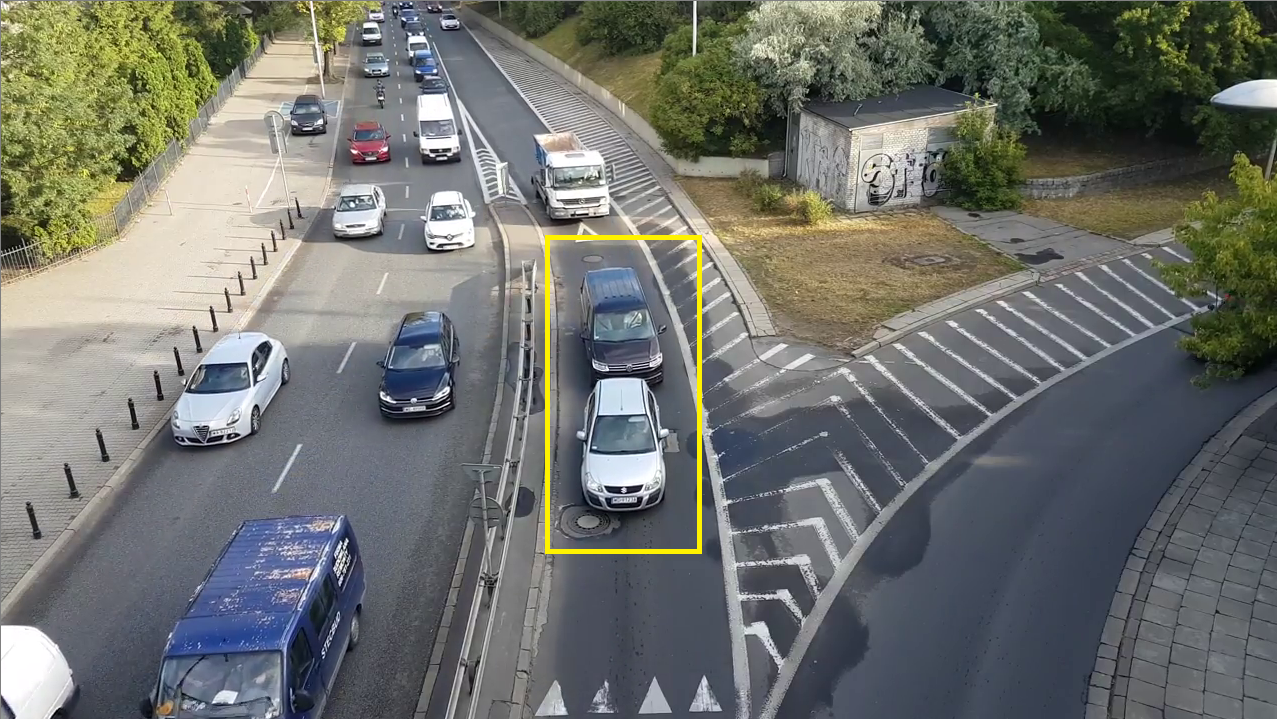
\includegraphics[width = 0.45\textwidth]{design/detection/calibration/original}
        \caption{}
        \label{fig:}
    \end{subfigure}%
    \begin{subfigure}[b]{0.5\linewidth}
        \centering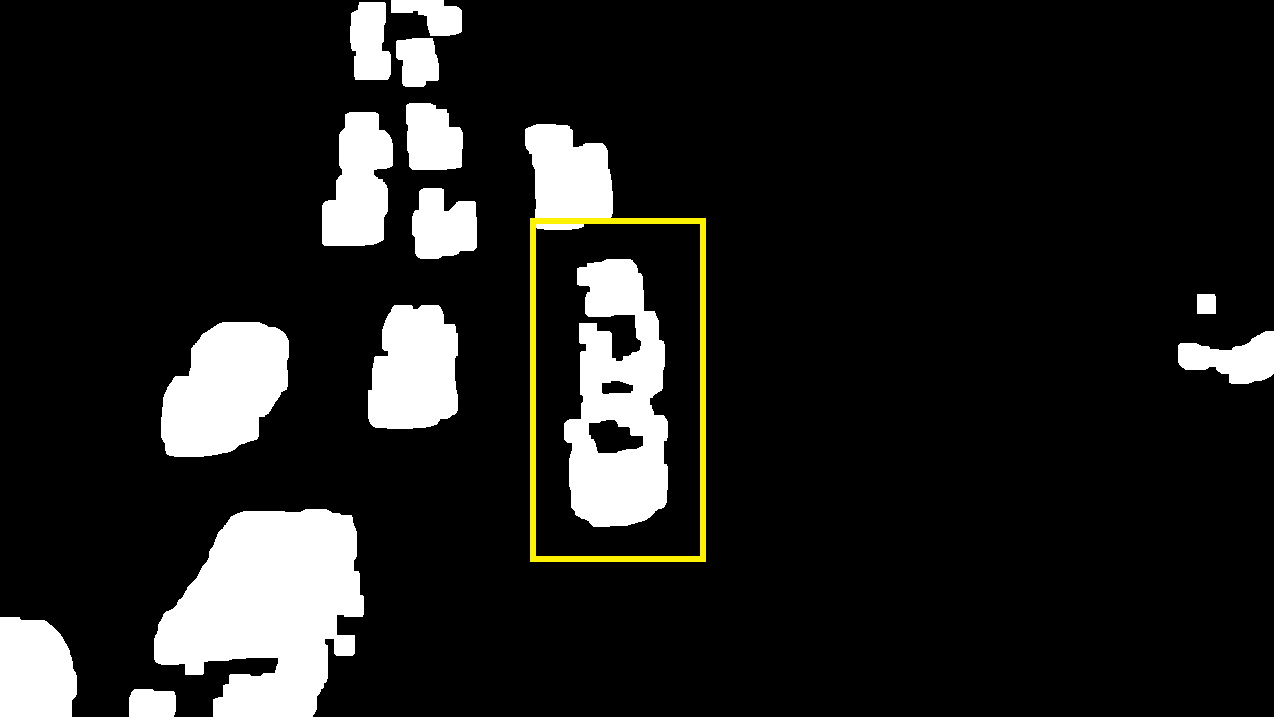
\includegraphics[width = 0.45\textwidth]{design/detection/calibration/mask}
        \caption{}
        \label{fig:}
    \end{subfigure}
    \begin{subfigure}[b]{0.5\linewidth}
        \centering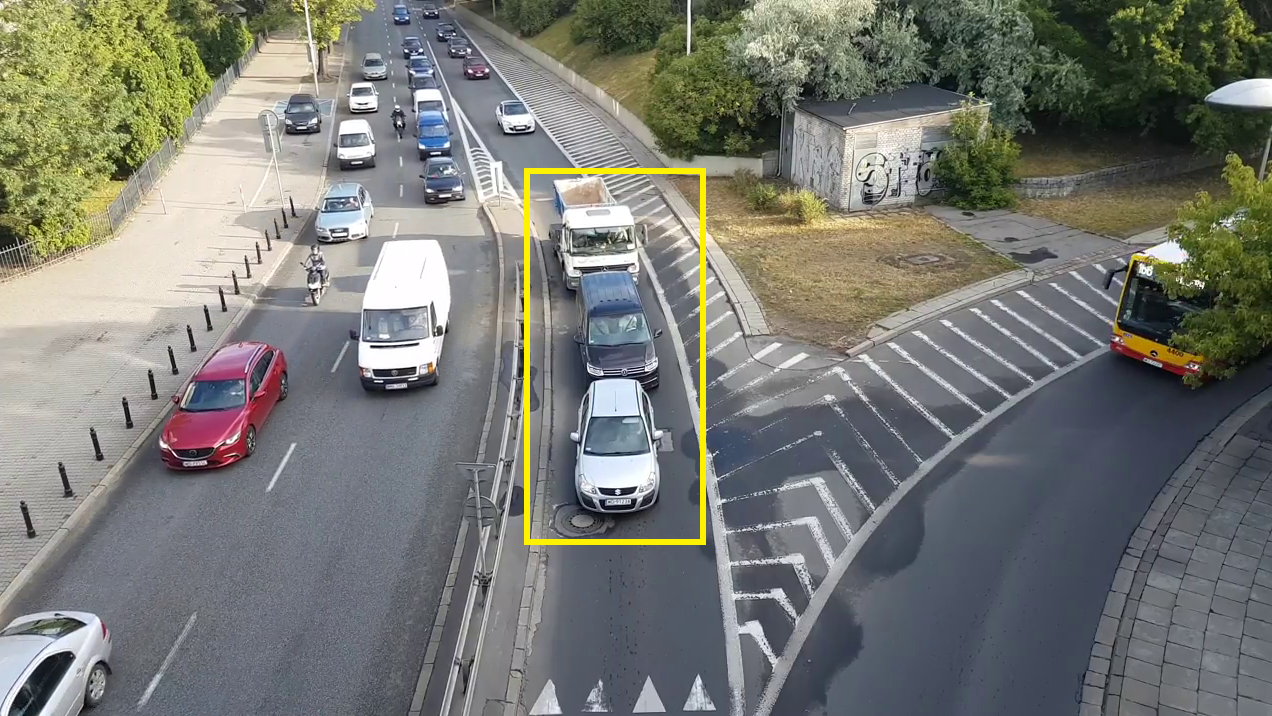
\includegraphics[width = 0.45\textwidth]{design/detection/calibration/original_adapted}
        \caption{}
		\label{fig:}
    \end{subfigure}%
    	\begin{subfigure}[b]{0.5\linewidth}
        \centering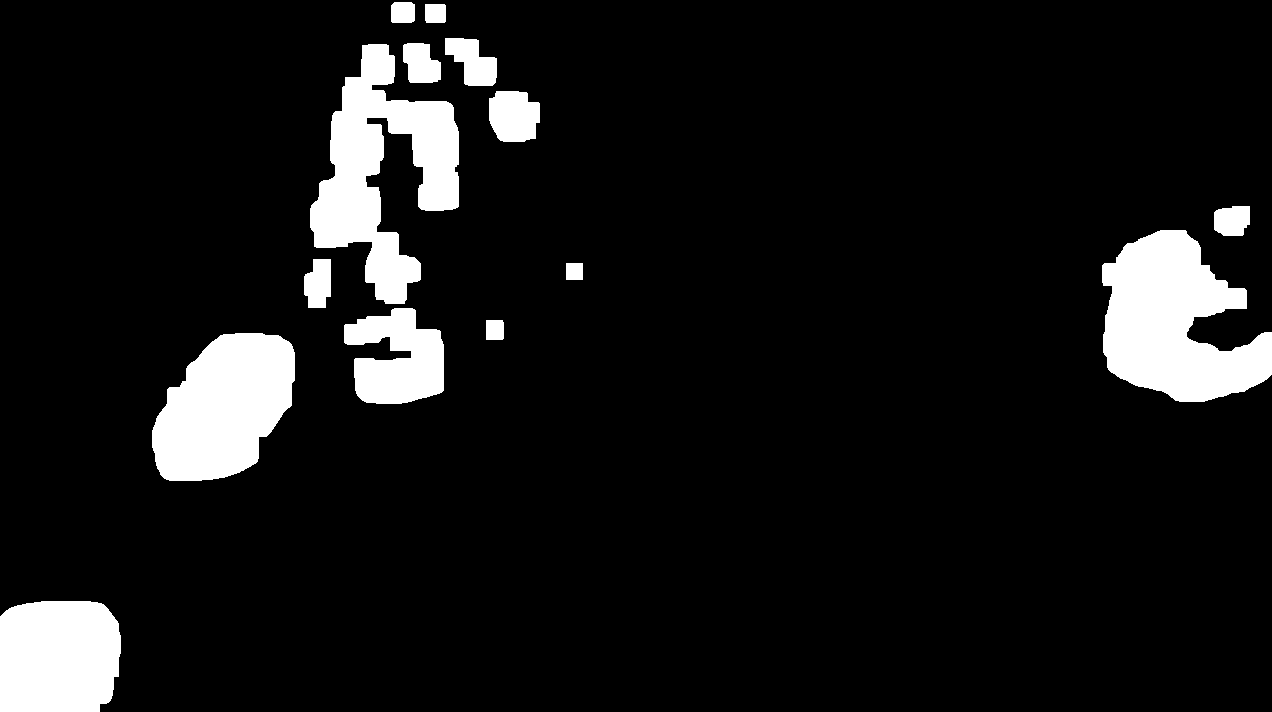
\includegraphics[width = 0.45\textwidth]{design/detection/calibration/mask_adapted}
        \caption{}
        \label{fig:}
    \end{subfigure}
    \caption{Adaptation of stationery vehicles in GMM background cluster. Video by Karol Majek}
    \label{fig:cluster_adaptation}
\end{figure}



\subsubsection{Morphological Operations and Filtering}

This is perhaps the most critical component of the calibration of the computer vision system as it is responsible for the consolidation of foreground objects which if not performed will leave fractured or anomolous entities that will be interpreted as vehicles and render the data obtained by the system as useless.This calibration is performed by visual analysis where the desired operations create connected components where they should exist and maintains separation where it should exist. 

The filtering component of this subprocess is trivial to calibrate as it should simply remove salt and pepper noise as in Figure \ref{fig:mask_saltnpepper}. Depending on the size of the individual noise entities, the size of the median filter should increased to ensure that the median value is background and the noise is removed. If the size of the noise entities is as large as the entities that should be maintained then the subtraction process requires revision. 

To find the optimal morphological structuring element shape and size, and the number of iterations of closing and dilation to perform requires greater testing than selecting a median filter. These operations can become computationally expensive depending on the size of the structuring element and number of iterations so minimising these factors is important. The purpose of morphing the foreground mask is to consolidate objects into connected components but also to ensure separation of entities if they don't belong to the same object which can be a delicate balance. The OpenCV function, \emph{exmorphology} provides three shapes of structuring element, ellipse, cross and rectangle, Figure \ref{fig:morph_testing} show a comparison of these shapes on the same foreground mask snapshot for a 7x7 element size and varying iterations. In observing the connection and separation of foreground entities, sometimes called blobs, the rectangular element on 3 iterations was selected. These settings are appropriate only for this scenario, i.e. this camera angle at this location and in a particular region of interest where vehicles are largest. In Figure \ref{fig:compare_closure} the closure of vehicle blobs in the region where traffic is closest to the camera are visually compared. In this case the blobs in the bounding boxes are closed successfully by the rectangular structuring element but not by the ellipse.


\begin{figure}[htbp]
    \centering
    \begin{subfigure}[b]{0.42\textwidth}
        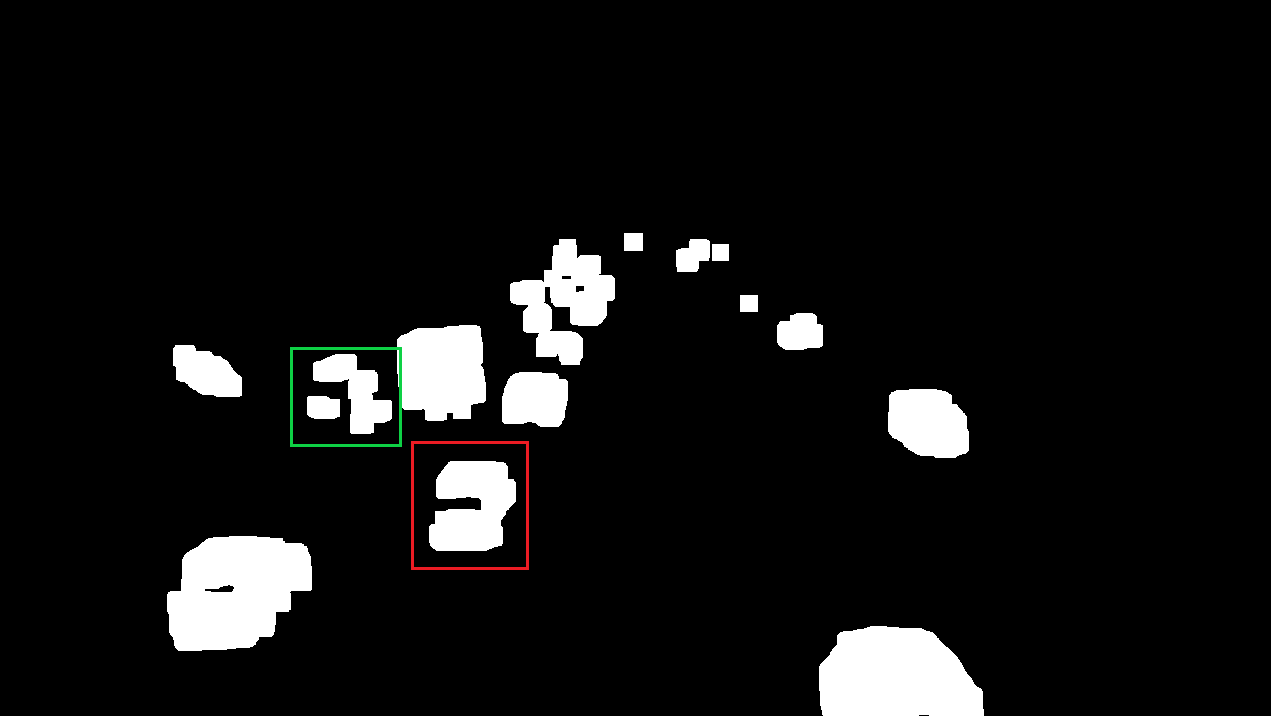
\includegraphics[width=\textwidth]{design/detection/calibration/rect_3_edit}
        \captionsetup{format = hang}
        \caption{Rectangular structuring element closure}
    \end{subfigure}
    \begin{subfigure}[b]{0.42\textwidth}
        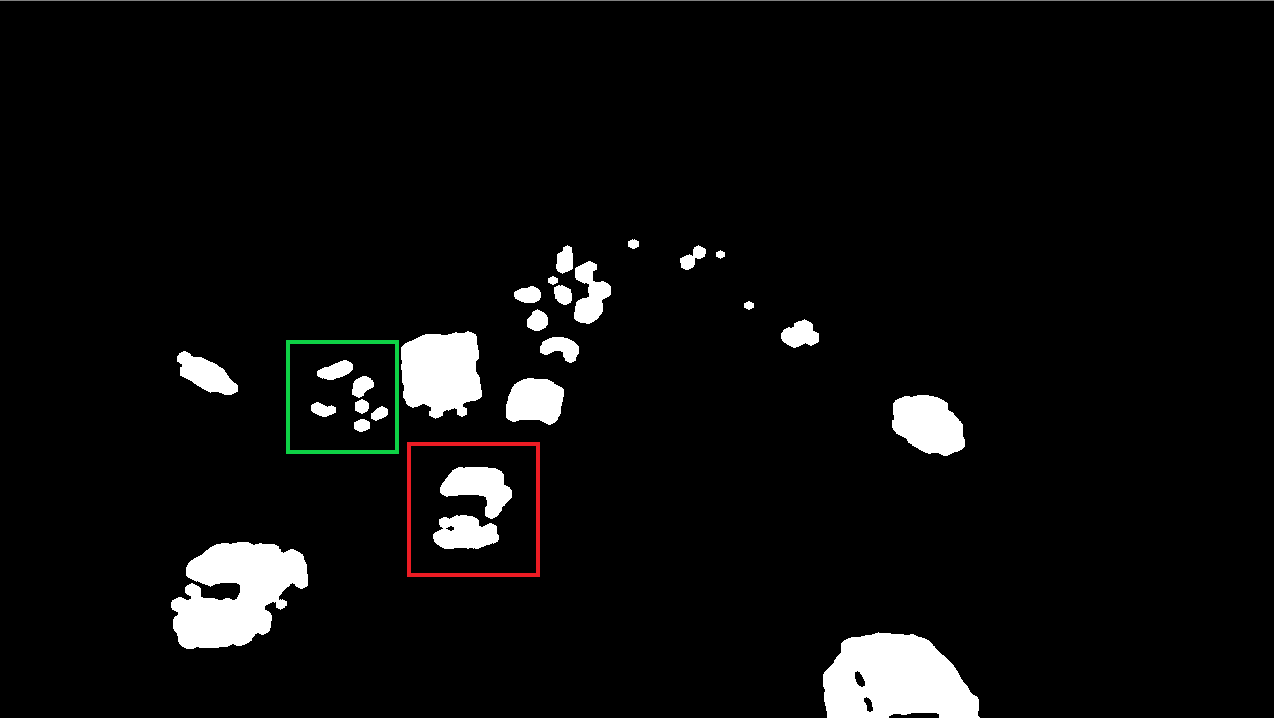
\includegraphics[width=\textwidth]{design/detection/calibration/ellipse_3_edit}
        \captionsetup{format = hang}
        \caption{Elliptical structuring element closure}
    \end{subfigure}
    \captionsetup{format = hang}
    \caption{Comparison of morphological closure using a 7x7 rectangular and elliptical structuring element for 3 iterations.}
    \label{fig:compare_closure}
\end{figure}


\begin{figure*}[htbp]
    \begin{tabular}{
        >{\centering\arraybackslash}m{0.4cm}
        >{\centering\arraybackslash}m{4.5cm}
        >{\centering\arraybackslash}m{4.5cm}
        >{\centering\arraybackslash}m{4.5cm}}
          & Ellipse & Cross & Rectangle \\
        1 
        &
        \begin{subfigure}[b]{0.3\textwidth}
            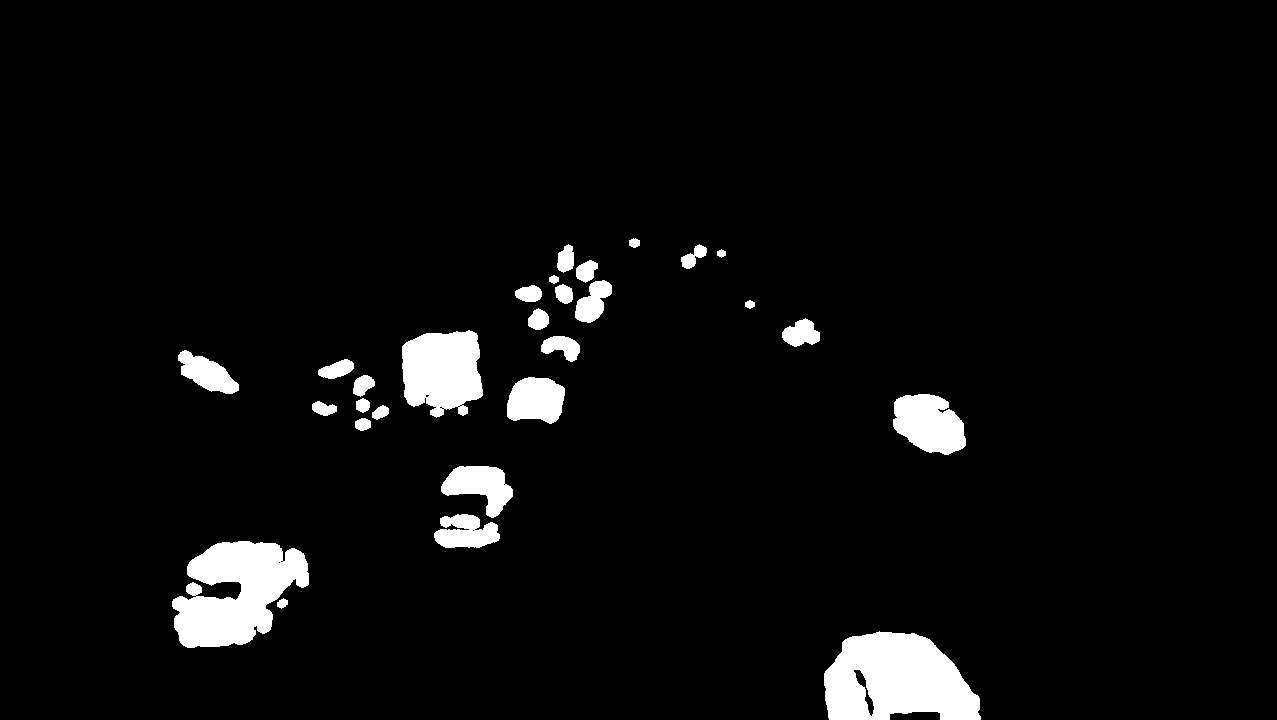
\includegraphics[width=\textwidth]{design/detection/morphology/ellipse_1}
            % \captionsetup{format = hang}
        \end{subfigure} &
        \begin{subfigure}[b]{0.3\textwidth}
            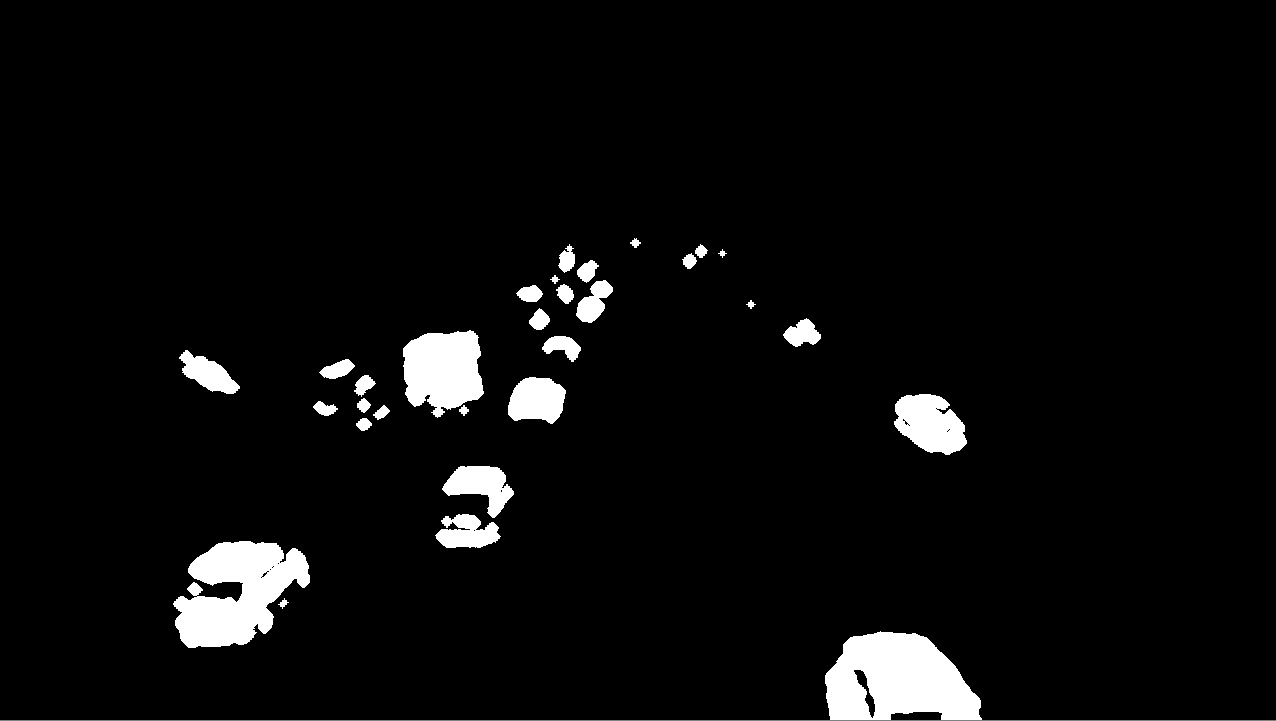
\includegraphics[width=\textwidth]{design/detection/morphology/cross_1}
            % \captionsetup{format = hang}
        \end{subfigure} &
        \begin{subfigure}[b]{0.3\textwidth}
            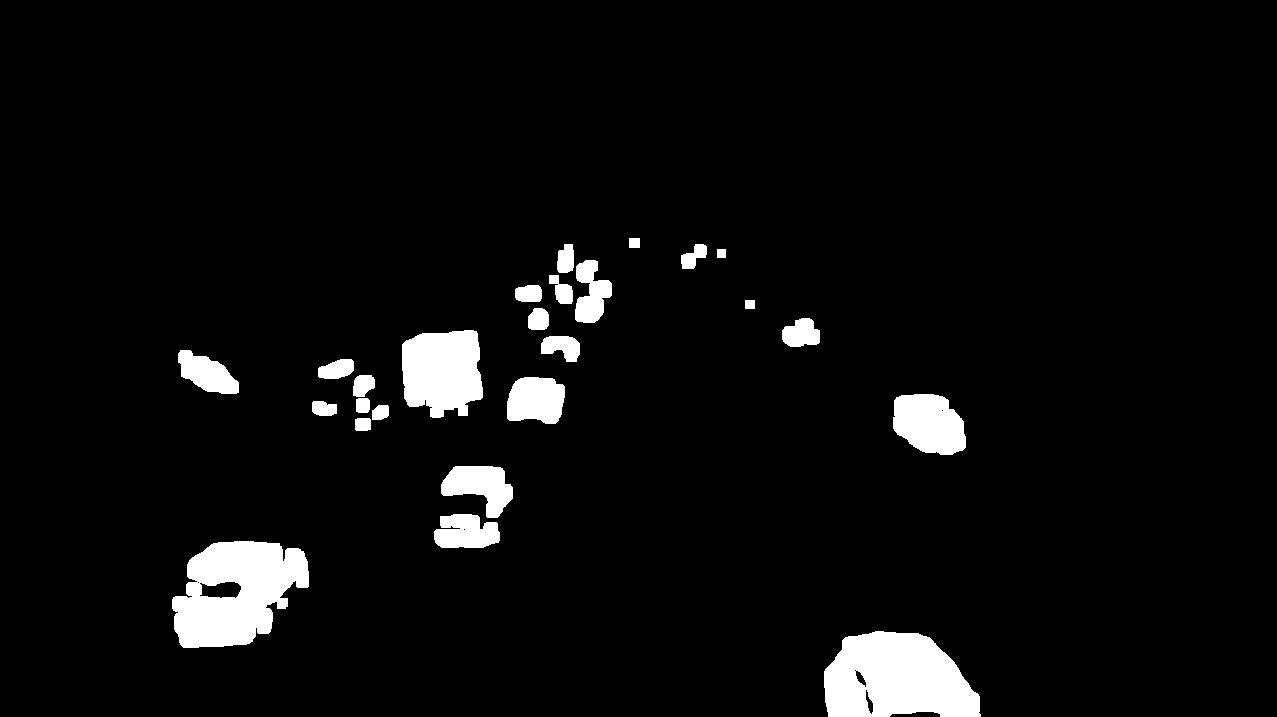
\includegraphics[width=\textwidth]{design/detection/morphology/rect_1}
            % \captionsetup{format = hang}
        \end{subfigure} \\
        3 &
        \begin{subfigure}[b]{0.3\textwidth}
            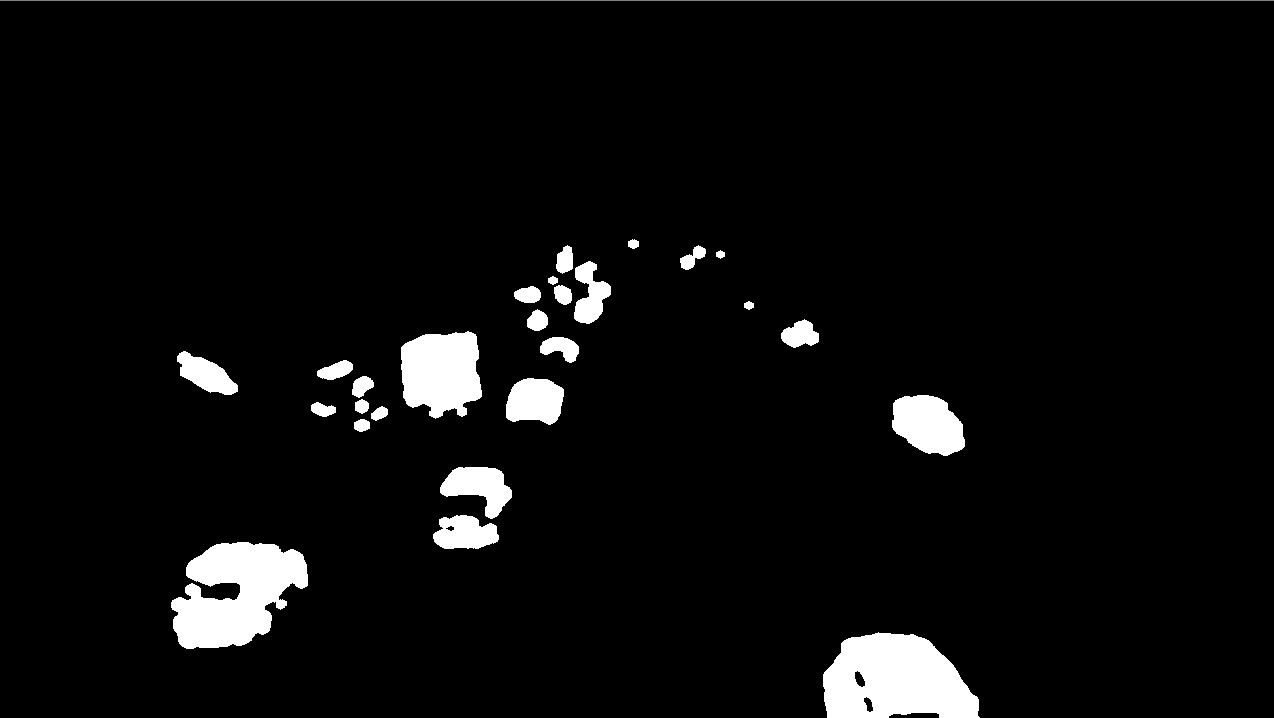
\includegraphics[width=\textwidth]{design/detection/morphology/ellipse_3}
            % \captionsetup{format = hang}
        \end{subfigure} &
        \begin{subfigure}[b]{0.3\textwidth}
            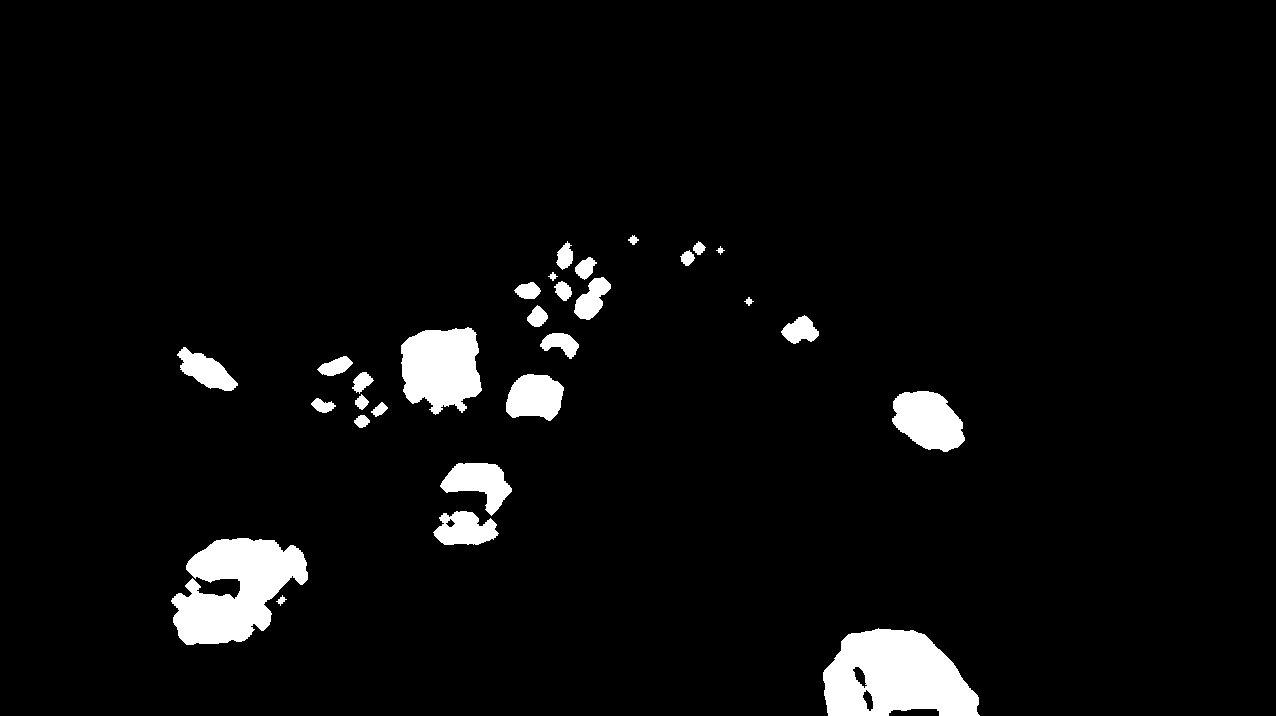
\includegraphics[width=\textwidth]{design/detection/morphology/cross_3}
            % \captionsetup{format = hang}
        \end{subfigure} &
        \begin{subfigure}[b]{0.3\textwidth}
            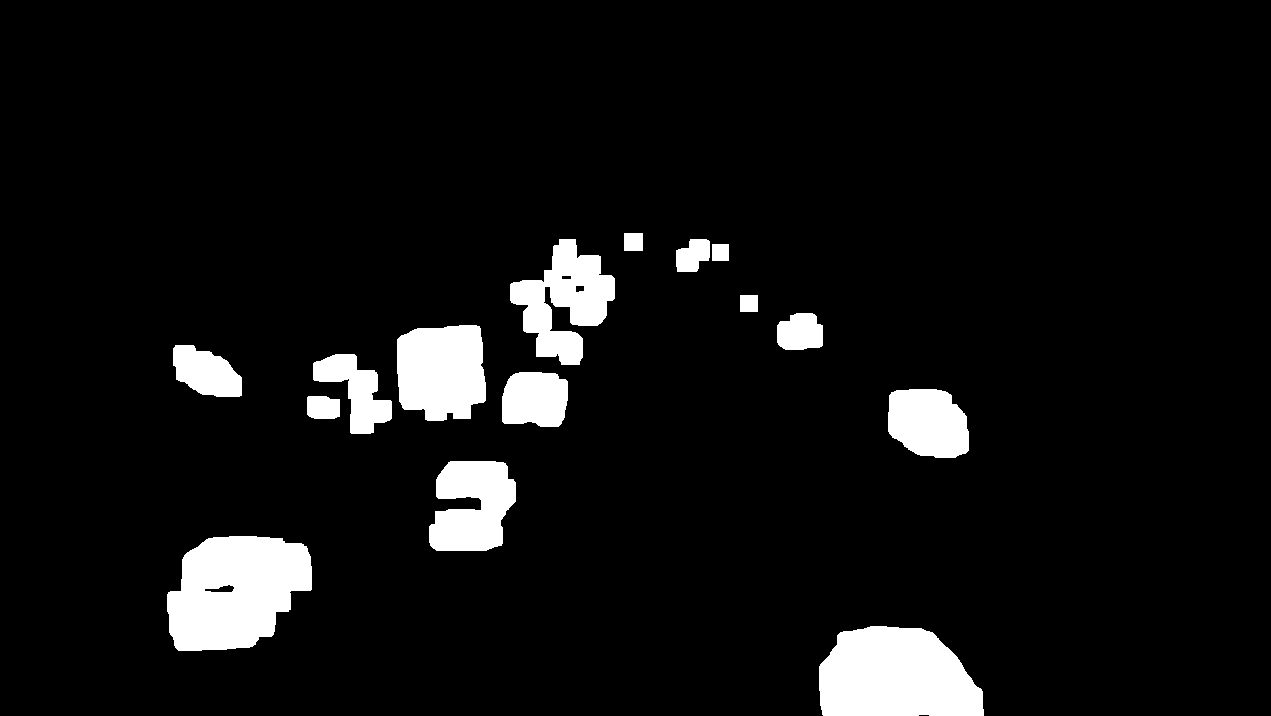
\includegraphics[width=\textwidth]{design/detection/morphology/rect_3}
            % \captionsetup{format = hang}
        \end{subfigure} \\
        5 &
        \begin{subfigure}[b]{0.3\textwidth}
            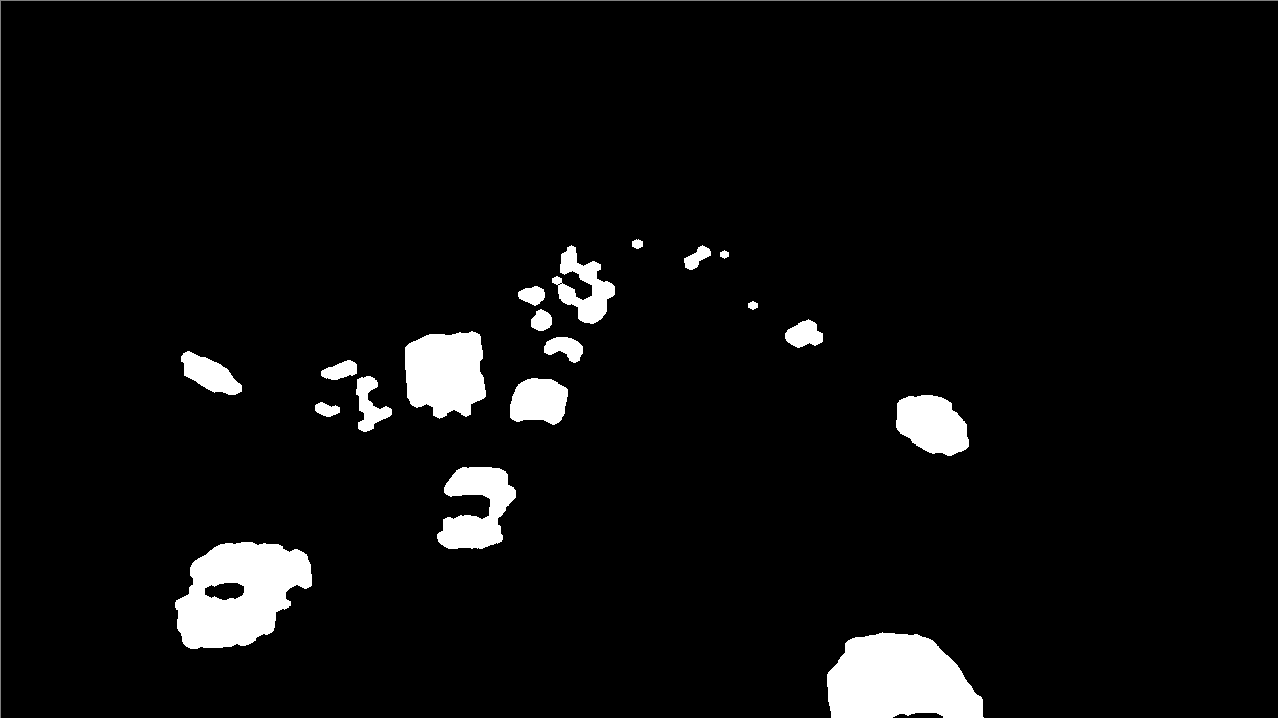
\includegraphics[width=\textwidth]{design/detection/morphology/ellipse_5}
            % \captionsetup{format = hang}
        \end{subfigure} &
        \begin{subfigure}[b]{0.3\textwidth}
            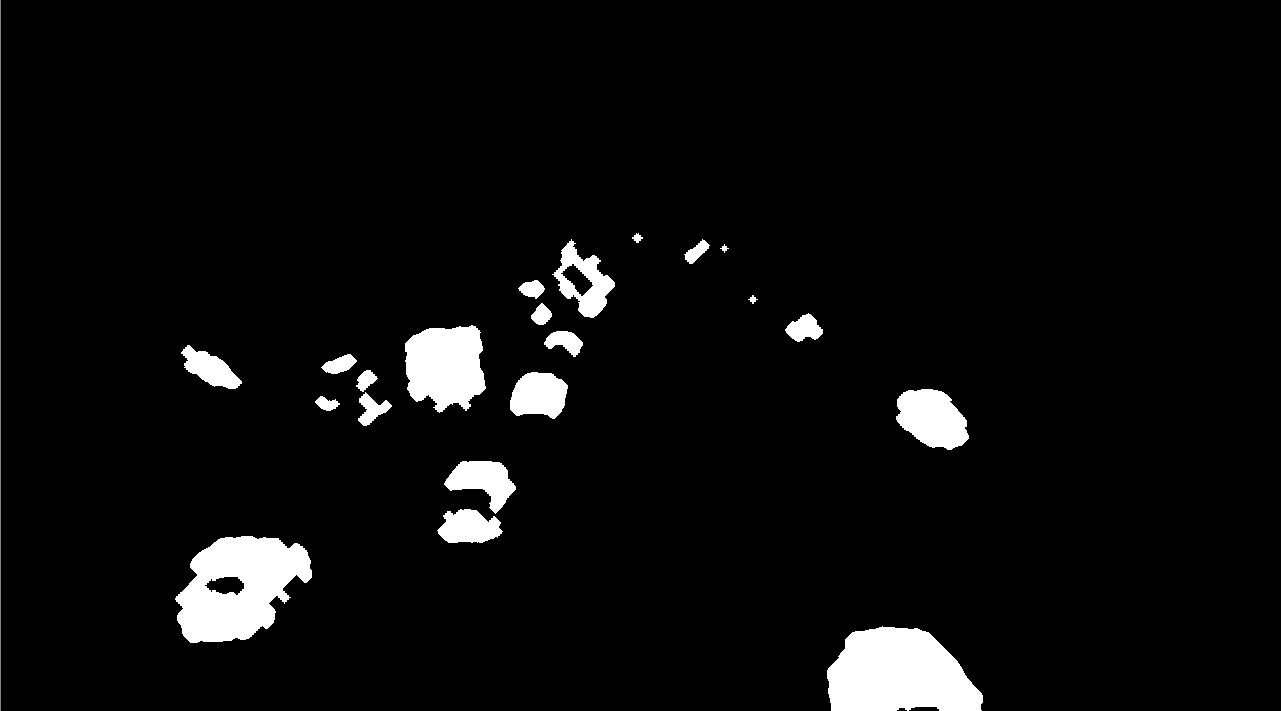
\includegraphics[width=\textwidth]{design/detection/morphology/cross_5}
            % \captionsetup{format = hang}
        \end{subfigure} &
        \begin{subfigure}[b]{0.3\textwidth}
            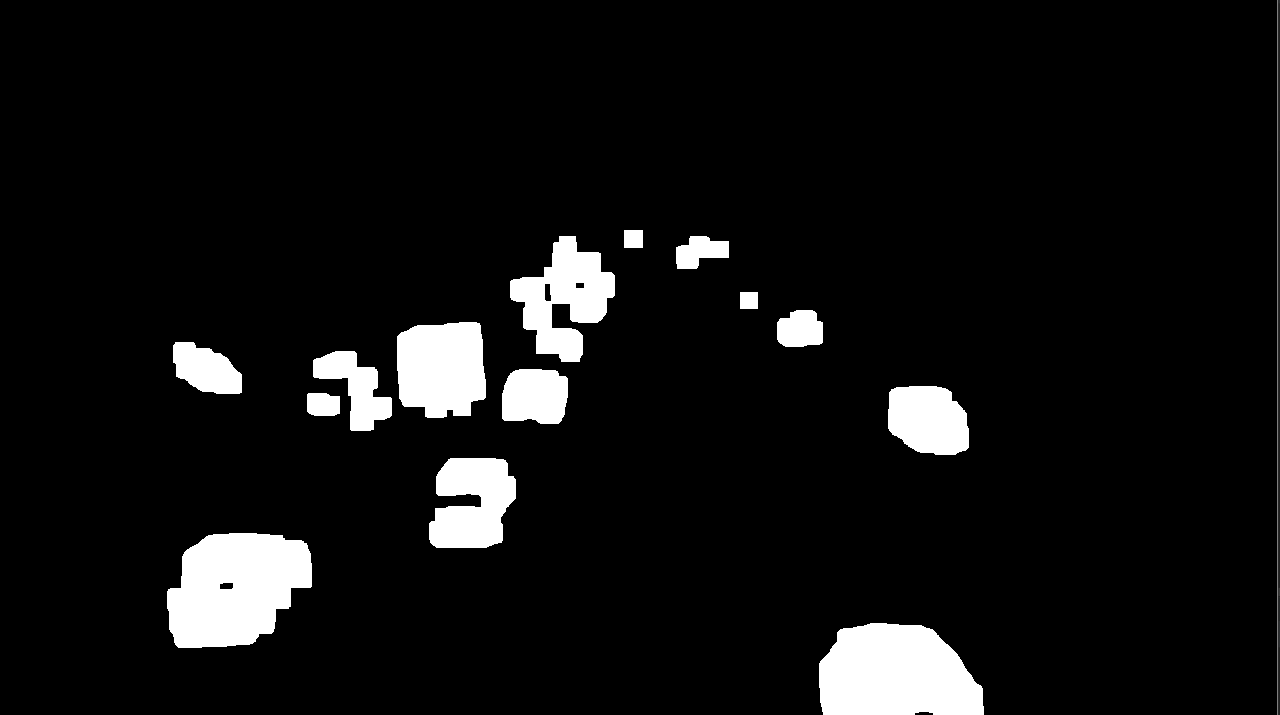
\includegraphics[width=\textwidth]{design/detection/morphology/rect_5}
            % \captionsetup{format = hang}
        \end{subfigure} \\
    \end{tabular}
    \captionsetup{format = hang}
    \caption{Morphological closing using different 7x7 structuring elements and iterations.}
    \label{fig:morph_testing}
\end{figure*}


\subsubsection{Bounding and Contours}


It's important yoooo....